
\section{Plotter}
Let us no use hepstores plotter to create figures of the scatter in
the x,y plane as well as histograms for the x and y axis. The command
we use is basically
%
\begin{changemargin}{1.5cm}{1.5cm} 
  \begin{lstlisting}[language=Bash]
    
    hepstore-plot -f data_1.npy data_2.npy -k scatter
    hepstore-plot -f data_1.npy data_2.npy -k histogram
  \end{lstlisting}
\end{changemargin}
%
%
\begin{figure}
  \centering
  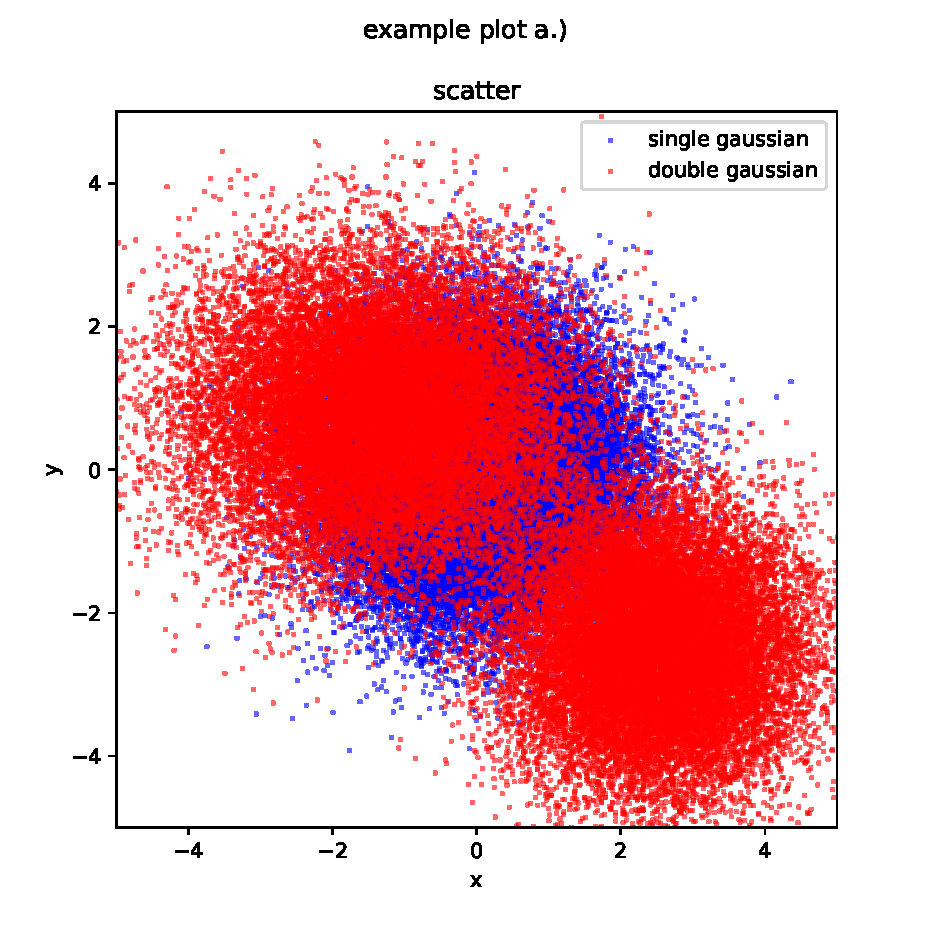
\includegraphics[width=0.32\textwidth]{../examples/core/plotter/example_a.pdf}
  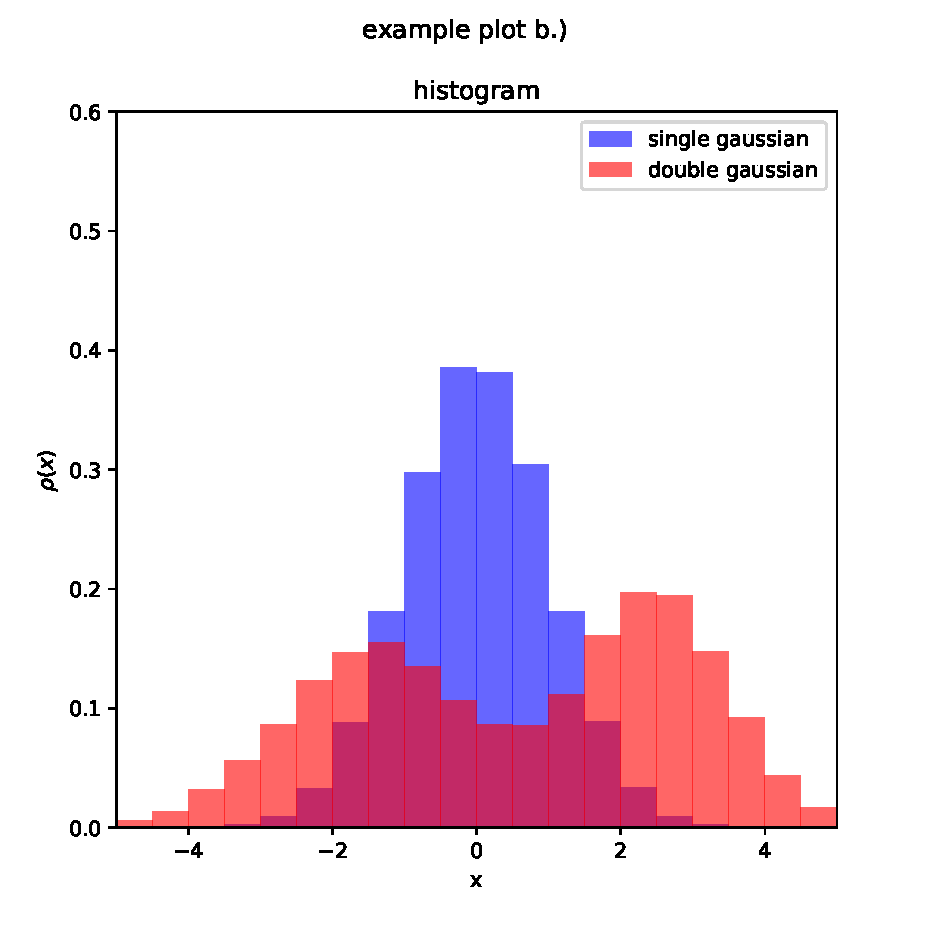
\includegraphics[width=0.32\textwidth]{../examples/core/plotter/example_b.pdf}
  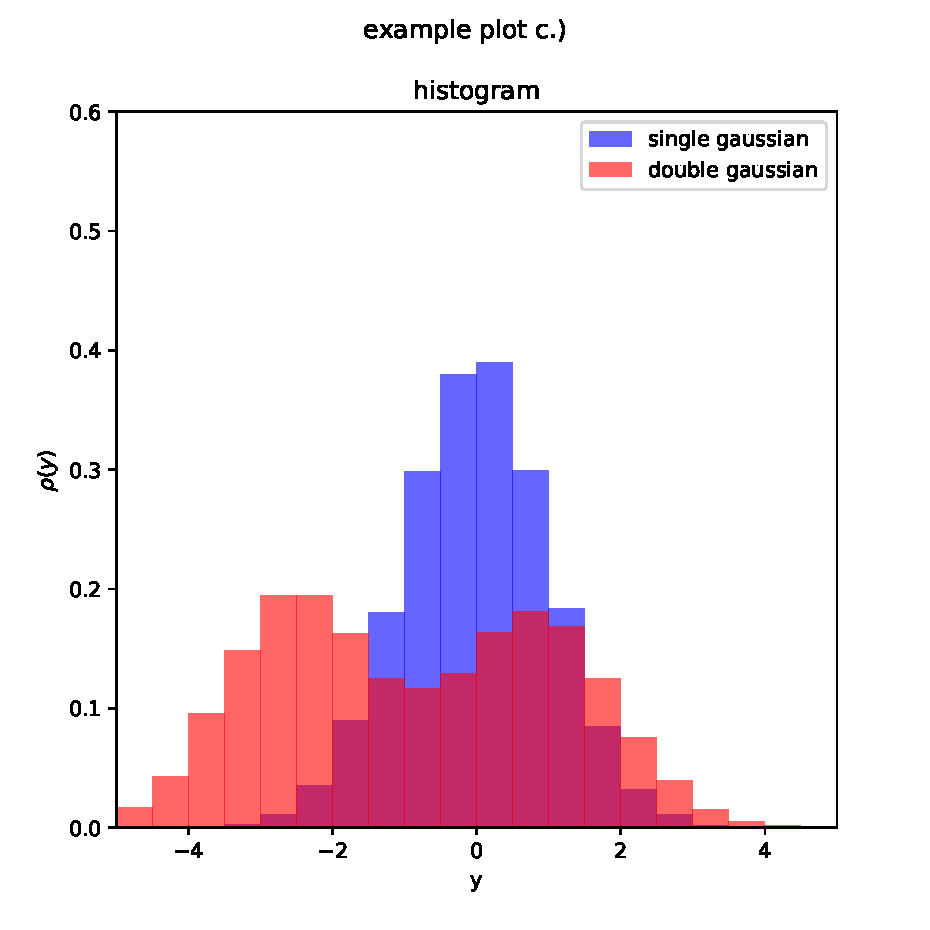
\includegraphics[width=0.32\textwidth]{../examples/core/plotter/example_c.pdf}
  \caption{}
  \label{fig:example_plotting}
\end{figure}
%
In Fig.~\ref{fig:example_plotting} we present the results obtained
with the srcipt from Sec.~\ref{sec:}. There finer steering arguments,
for example colors and labels, have been used.


